% array pile
\documentclass[12pt,letterpaper,oneside,titlepage]{article}
\usepackage[latin1]{inputenc}
\usepackage{amsmath}
\usepackage{amsfonts}
\usepackage{amssymb}
\usepackage{graphicx}
\usepackage[letterpaper, portrait, margin=.5in]{geometry}
\usepackage{lscape}
\usepackage{tikz}
\usetikzlibrary{matrix,calc}
\usepackage{color}
\usepackage{tabto}
\usepackage{pgfplots}

%\usepackage[table]{xcolor}% http://ctan.org/pkg/xcolor



\begin{document}
	\author{Scott \textbf{``Cash''} Fields}
	\title{GRAPHS}
	
	%%%%%   LEARN     %%%%%%%%%%%%%%%%%%%%%
	%%%%%%%%%%%%%%%%%%%%%%%%%%%%%%%%
	
	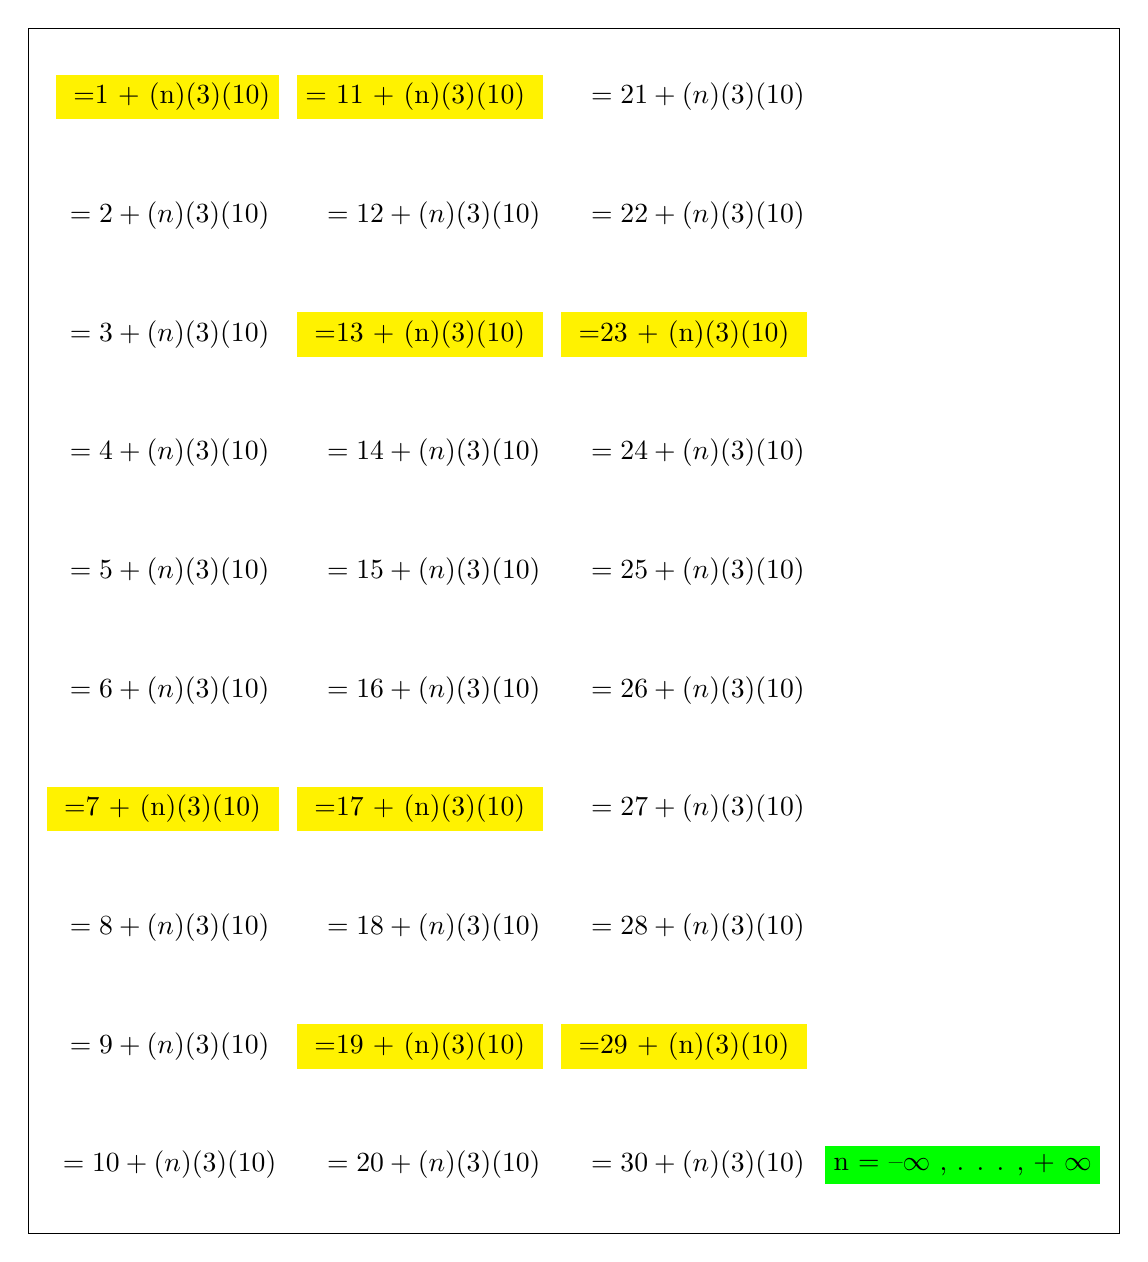
\begin{tikzpicture}[every node/.style={anchor=north east ,fill=white,minimum width=3cm,minimum height=15mm}]

	\matrix (mA) [draw,matrix of math nodes]
{
		\colorbox{yellow}{ =1 + (n)(3)(10)}   &   \colorbox{yellow}{= 11 + (n)(3)(10) }   &     =21 + (n)(3)(10)   &    \\
		=2 + (n)(3)(10)   &   =12 + (n)(3)(10)    &     =22 + (n)(3)(10)   &    \\
		=3 + (n)(3)(10)   &   \colorbox{yellow}{ =13 + (n)(3)(10) }   &   	\colorbox{yellow}{ =23 + (n)(3)(10) }  &    \\
		=4 + (n)(3)(10)   &   =14 + (n)(3)(10)    &     =24 + (n)(3)(10)   &    \\
		=5 + (n)(3)(10)   &   =15 + (n)(3)(10)    &     =25 + (n)(3)(10)   &    \\
		=6 + (n)(3)(10)   &   =16 + (n)(3)(10)    &     =26 + (n)(3)(10)   &    \\
		\colorbox{yellow}{ =7 + (n)(3)(10) }   &   \colorbox{yellow}{ =17 + (n)(3)(10) }    &     =27 + (n)(3)(10)   &    \\
		=8 + (n)(3)(10)   &   =18 + (n)(3)(10)    &     =28 + (n)(3)(10)   &    \\
		=9 + (n)(3)(10)   &   \colorbox{yellow}{ =19 + (n)(3)(10) }    &     \colorbox{yellow}{ =29 + (n)(3)(10) }   &    \\
		=10 + (n)(3)(10)  &   =20 + (n)(3)(10)   &     =30 + (n)(3)(10)    &  
		\colorbox{green}{n = \textendash $\infty$ , . . . ,  + $\infty$} \\
};
	
		
	
	\pagebreak
	\end{tikzpicture}
	\pagebreak
	
	
	
	
	%%%%%%%%%%%%%%%%%%%%%%%%%%%%%%%%%%


	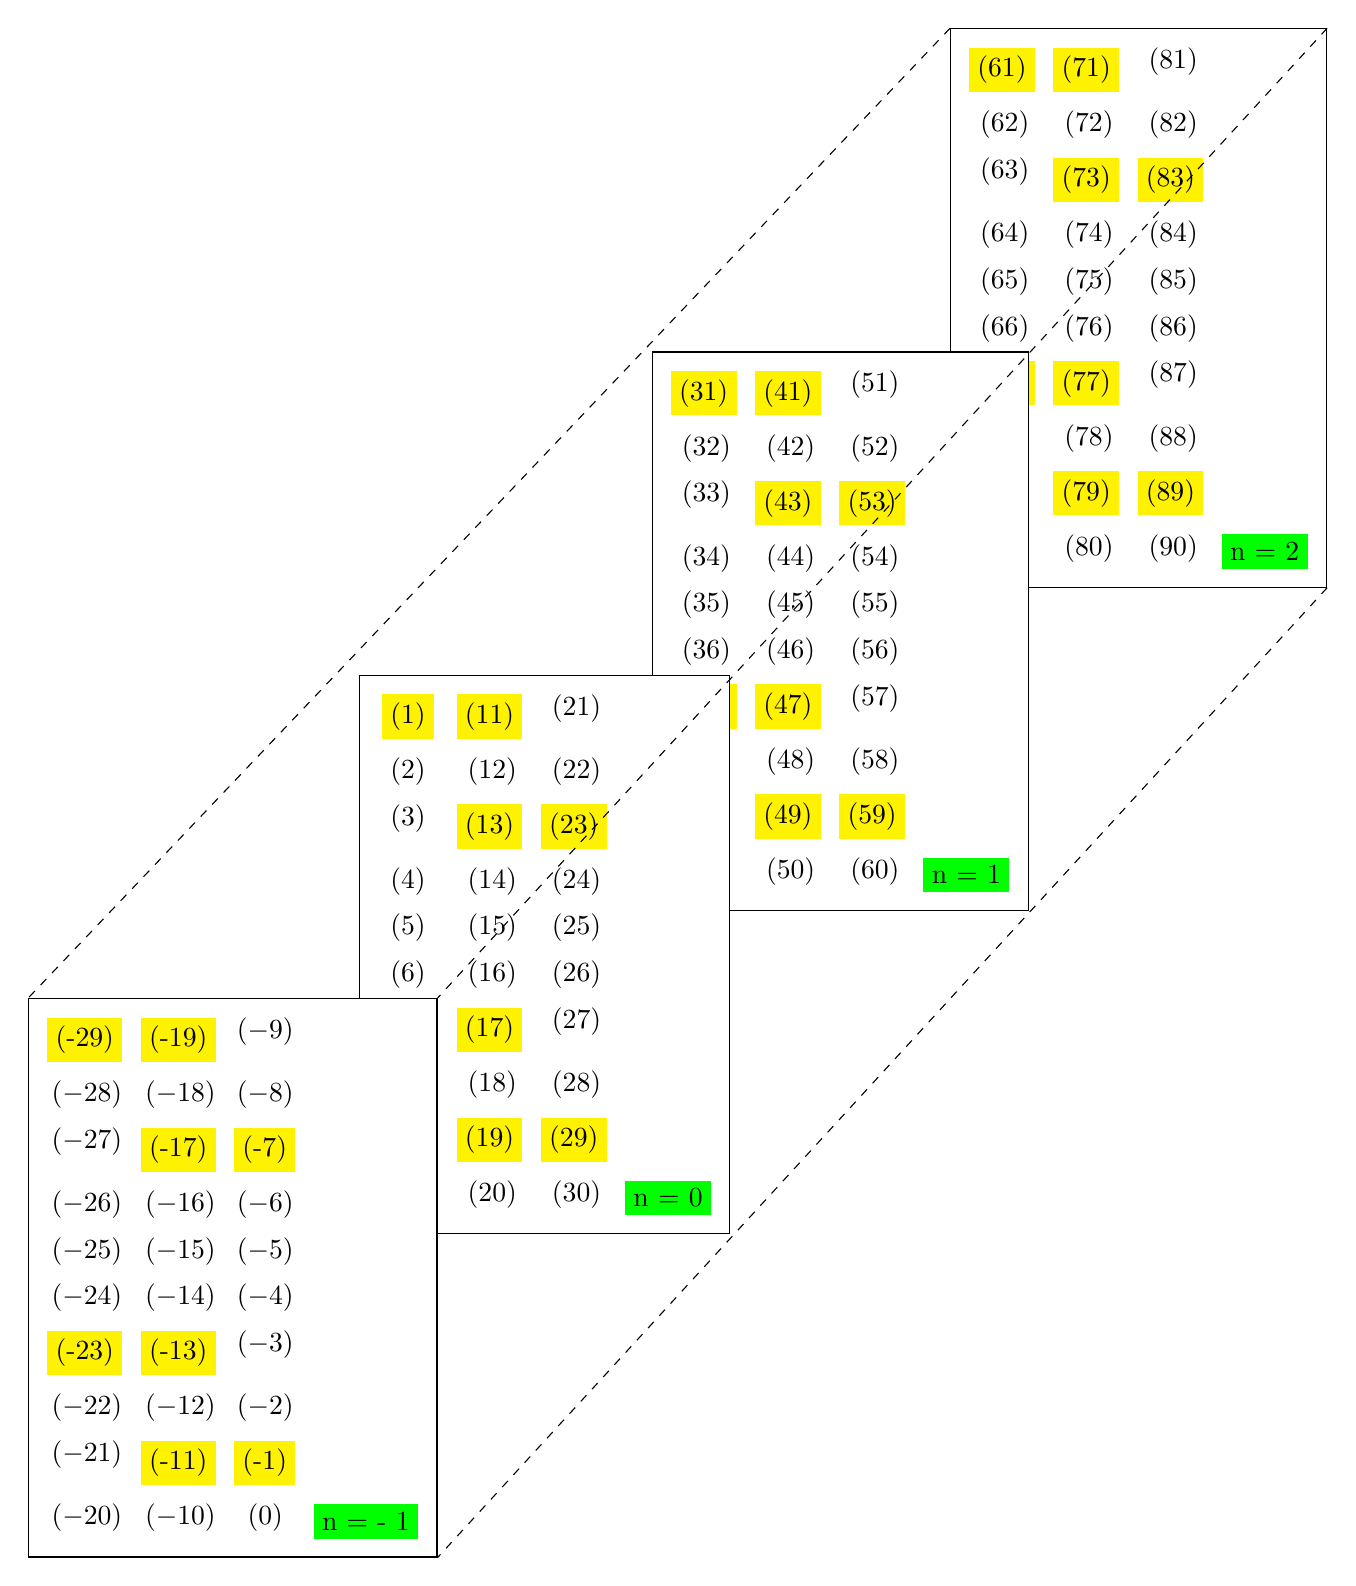
\begin{tikzpicture}[every node/.style={anchor=north east ,fill=white,minimum width=1cm,minimum height=5mm}]
	
	\matrix (mA) [draw,matrix of math nodes]
        {
        \colorbox{yellow}{(61)}   & \colorbox{yellow}{(71)} & (81)  &  \\
%        (61)   & (71) & (81)  &  \\
		(62)   & (72) & (82)  &  \\ 
		(63)   & \colorbox{yellow}{(73)} & \colorbox{yellow}{(83)}  &  \\        
%		(63)   & (73) & (83)  &  \\        
		(64)   & (74) & (84)  &  \\        
		(65)   & (75) & (85)  &  \\        
		(66)   & (76) & (86)  &  \\
		\colorbox{yellow}{(67)}   & \colorbox{yellow}{(77)} & (87)  &  \\        
%		(67)   & (77) & (87)  &  \\        
		(68)   & (78) & (88)  &  \\ 
		(69)   & \colorbox{yellow}{(79)} & \colorbox{yellow}{(89)}  &  \\       
%		(69)   & (79) & (89)  &  \\        
		(70)   & (80) & (90)  &  \colorbox{green}{n = 2} \\ 
		};

	
	\matrix (mB) [draw,matrix of math nodes] at ($(mA.south west)+(1,3)$)
        {
        \colorbox{yellow}{(31)}   & \colorbox{yellow}{(41)} & (51)  &  \\        
 %       (31)   & (41) & (51)    &  \\
		(32)   & (42) & (52)    &  \\
		(33)   & \colorbox{yellow}{(43)} & \colorbox{yellow}{(53)}  &  \\    
%		(33)   & (43) & (53)    &  \\
		(34)   & (44) & (54)    &  \\
		(35)   & (45) & (55)    &  \\
		(36)   & (46) & (56)    &  \\
		\colorbox{yellow}{(37)}   & \colorbox{yellow}{(47)} & (57)  &  \\
%		(37)   & (47) & (57)    &  \\
		(38)   & (48) & (58)    &  \\
		(39)   & \colorbox{yellow}{(49)} & \colorbox{yellow}{(59)}  &  \\
%		(39)   & (49) & (59)    &  \\
		(40)   & (50) & (60)    & \colorbox{green}{n = 1} \\  
	};  
	
	\matrix (mC) [draw,matrix of math nodes] at ($(mB.south west)+(1,3)$)
	{
        \colorbox{yellow}{(1)}   & \colorbox{yellow}{(11)} & (21)  &  \\        
		(2)   & (12) & (22)  &  \\        
		(3)   & \colorbox{yellow}{(13)} & \colorbox{yellow}{(23)}  &  \\        
		(4)   & (14) & (24)  &  \\        
		(5)   & (15) & (25)  &  \\        
		(6)   & (16) & (26)  &  \\        
		\colorbox{yellow}{(7)}   & \colorbox{yellow}{(17)} & (27)  &  \\        
		(8)   & (18) & (28)  &  \\        
		(9)   & \colorbox{yellow}{(19)} & \colorbox{yellow}{(29)}  &  \\        
		(10) & (20) & (30) &  \colorbox{green}{n = 0} \\  
	};
	
	
	\matrix (mD) [draw,matrix of math nodes] at ($(mC.south west)+(1,3)$)	
        {
       \colorbox{yellow}{(-29)}   & \colorbox{yellow}{(-19)} & (-9)  &  \\      
%	(-29)   & (-19) & (-9) &  \\
	(-28)   & (-18) & (-8) &  \\
	(-27)   & \colorbox{yellow}{(-17)} & \colorbox{yellow}{(-7)}  &  \\    
%	(-27)   & (-17) & (-7) &  \\
	(-26)   & (-16) & (-6) &  \\
	(-25)   & (-15) & (-5) &  \\
	(-24)   & (-14) & (-4) &  \\
	\colorbox{yellow}{(-23)}   & \colorbox{yellow}{(-13)} & (-3)  &  \\        
%	(-23)   & (-13) & (-3) &  \\
	(-22)   & (-12) & (-2) &  \\
	(-21)   & \colorbox{yellow}{(-11)} & \colorbox{yellow}{(-1)}  &  \\        
%	(-21)   & (-11) & (-1) &  \\
	(-20)   & (-10) & (0)  &  \colorbox{green}{n = - 1} \\
};                                   
	
	

	\draw[dashed](mA.north east)--(mD.north east);
	\draw[dashed](mA.north west)--(mD.north west);
	\draw[dashed](mA.south east)--(mD.south east);


	\pagebreak
	\end{tikzpicture}
	\pagebreak
	
\end{document}
